\documentclass[11pt]{article}
\usepackage[margin=1in]{geometry}
\usepackage{amsmath,amssymb}
\usepackage{graphicx}
\usepackage{booktabs}
\usepackage{hyperref}
\usepackage{xcolor}
\usepackage{caption}
\usepackage{placeins}

\title{Joint Calibration: Reproducing Roughness, the Leverage Effect,\\
the Taylor Effect, the Zumbach Effect, and Excess Kurtosis\\
Simultaneously, Per Asset}
\author{Companion note to the ESN A2-981003 market-data hyperparameter search}
\date{September 5, 2026}

\begin{document}
\maketitle

\begin{abstract}
Every note in this family so far has calibrated the ESN--A2 architecture to
\emph{one} stylised fact at a time. This note calibrates all 5 --
roughness (the moment-based Hurst exponent), the leverage effect, the
Taylor effect, the Zumbach effect, and excess kurtosis -- simultaneously,
per asset, via a single combined objective and a 6-parameter search
$\theta=(H,\texttt{rough\_scale},\lambda_{lo},\lambda_{hi},m_1,\alpha)$.
$\alpha$ is a feedback layer: the raw pre-activation variance feeds an
EWMA recursion producing a 2nd, smoothed signal that recursively depends
on its own previous value, used to generate returns (giving Taylor and
kurtosis genuine multi-day persistence) while Hurst, leverage, and
Zumbach all read the unsmoothed signal directly. Each lag-indexed
statistic is additionally smoothed with a light 3-point moving average
across adjacent lags before entering the residual, applied identically to
the ESN's own simulated curve and the real target curve; Taylor's own 2
curves are fit separately (not their difference) and Zumbach on its own
raw level (not shape-normalised), neither carrying an extra weight
multiplier. A 2nd, independent fix corrects the optimiser itself: freezing
the random seed within each calibration run (common random numbers)
produced clean, monotonic convergence for every asset. Combined,
roughness and kurtosis are essentially perfect ($9/9$), leverage remains
excellent, and -- the central result of this note -- the Taylor effect,
which collapsed to a strict $0\%$ floor without the feedback layer,
recovers to $33$--$100\%$ coverage for 8 of 9 assets; the Zumbach effect's
own qualitative shape (rising vs.\ falling with horizon) is also
substantially more often correct. \texttt{RUSSELL2000} is the one clear
exception, regressing on Taylor and Zumbach under this combination.
\end{abstract}

\tableofcontents

\section{Motivation and set-up}
The 9-asset bench is the same throughout this note family: 6 stocks
(\texttt{LHX}, \texttt{BK}, \texttt{HUM}, \texttt{TSN}, \texttt{IEX},
\texttt{KMB}) and 3 indices (\texttt{SP500}, \texttt{RUSSELL2000},
\texttt{NASDAQ100}). Real targets for leverage, Taylor, Zumbach, and
kurtosis are taken directly from those notes' own computations; the real,
bias-corrected moment-based Hurst exponent is computed fresh for this same
bench. $N_r=22,N_z=29$ and the 7 shared $z$-bank hyperparameters are fixed
at the companion note's own optimum throughout.

\section{The model}
\label{sec:model}
The simulator is a 2-layer echo-state network: a linear reservoir of
Ornstein--Uhlenbeck modes, and a nonlinear $z$-bank reading 2 taps off the
reservoir, with a feedback-layer split of the resulting variance signal.

\subsection{The reservoir}
$r_t=(r_{t,1},\dots,r_{t,N_r})$ is a bank of independent
Ornstein--Uhlenbeck processes with geometrically spaced rates,
\begin{equation}
\lambda_i = \lambda_{lo}\Big(\frac{\lambda_{hi}}{\lambda_{lo}}\Big)^{
\frac{i-1}{N_r-1}}\, ,\qquad i=1,\dots,N_r\, ,
\label{eq:lambdas}
\end{equation}
updated once per day ($dt=1$) from a single shared innovation
$\varepsilon_t\sim\mathcal N(0,1)$:
\begin{equation}
r_{t+1,i} = \alpha_i^{\text{OU}}\,r_{t,i} + c_i\,\varepsilon_t\, ,
\qquad \alpha_i^{\text{OU}}=e^{-\lambda_i dt}\, ,\qquad
c_i=\sqrt{1-(\alpha_i^{\text{OU}})^2}\, ,
\label{eq:reservoirupdate}
\end{equation}
(the reservoir's own per-mode decay $\alpha_i^{\text{OU}}$ is unrelated to
the calibrated feedback parameter $\alpha$ of \S\ref{sec:feedback}). The
reservoir is read through a single fixed direction $q\in\mathbb R^{N_r}$,
$q_i\propto\lambda_i^{0.5-H}$, unit-normalised and then
variance-normalised against the reservoir's own stationary autocovariance
so that $q^\top C q=1$.

\subsection{The $z$-bank}
$z_t=(z_{t,1},\dots,z_{t,N_z})$ is a nonlinear bank with its own
geometrically spaced decay rates. Each unit reads 2 fixed reservoir taps,
$p_1=r_{t+1,\text{fast}(j)}$, $p_2=r_{t+1,\text{slow}(j)}$:
\begin{equation}
z_{t+1,j} = e^{-a_j dt}z_{t,j} + \big(1-e^{-a_j dt}\big)\,
m_{t+1}\,\texttt{z\_strength}\,\tanh(u_{t,j})\, ,
\label{eq:zupdate}
\end{equation}
\begin{equation}
\begin{split}
u_{t,j} = {}& s_j p_1 p_2 + \texttt{even\_strength}\big(0.7p_1^2+0.3p_2^2-1\big)
-\texttt{linear\_strength}\big(0.7p_1+0.3p_2\big) \\
&+\texttt{zz\_scale}_j\,z_{t,j} + \tfrac12\texttt{local\_z\_strength}
\big(z_{t,j-1}+z_{t,j+1}\big)\, ,
\end{split}
\label{eq:udef}
\end{equation}
with the gate $m_{t+1}=\max\!\big(0,\,1-\texttt{gamma\_norm}\,
\lVert r_{t+1}\rVert/\sqrt{N_r}\big)$ suppressing the $z$-bank's own
update whenever the reservoir's current norm is large.

\subsection{Pre-activation and the feedback layer}
\label{sec:feedback}
Using $r_t,z_t$ (the state before this step's own update),
\begin{equation}
\eta_t = b_0 + \rho_r\,\texttt{rough\_scale}\,(q^\top r_t)
+ \sum_{j=1}^{N_z} w_{j,z}\,z_{j,t}
+ \frac{1}{N_r}\Big(m_1\lVert r_t\rVert^2 + m_2(q^\top r_t)^2\Big)\, ,
\label{eq:eta}
\end{equation}
$m_2$ held fixed at $0$; only $m_1$ calibrated. The raw pre-activation
variance is
\begin{equation}
(\sigma_t^{\text{raw}})^2 = \text{SIG\_MIN}^2+\text{softplus}(\eta_t)^2\, ,
\label{eq:sigrawdef}
\end{equation}
which feeds a genuine feedback layer -- an EWMA recursion depending on its
own previous value, not just on $\sigma_t^{\text{raw}}$:
\begin{equation}
(\sigma_t^{\text{used}})^2 = (1-\alpha)(\sigma_{t-1}^{\text{used}})^2
+\alpha(\sigma_t^{\text{raw}})^2\, .
\label{eq:sigused}
\end{equation}
Daily log-returns are generated from $\sigma_t^{\text{used}}$,
$dX_t=-\tfrac12(\sigma_t^{\text{used}})^2+\sigma_t^{\text{used}}
\varepsilon_t$ (reusing the same $\varepsilon_t$ that updates $r_{t+1}$).
$\alpha=1$ recovers $\sigma_t^{\text{used}}\equiv\sigma_t^{\text{raw}}$
exactly (verified bit-identical), i.e.\ a single, unsmoothed signal.
Hurst, leverage, and Zumbach all read $\sigma_t^{\text{raw}}$ directly (an
EWMA is itself autocorrelated, and was found to inject a spurious
dip-and-recovery shape into leverage's own $\text{corr}(x_t,v_{t+L})$ when
read from a smoothed signal); Taylor and kurtosis, functions of returns
alone, inherit whatever persistence the feedback layer injects into
$X_t$.

\paragraph{Interpretation.} $\sigma_t^{\text{raw}}$ is the reservoir's own
\emph{instantaneous} read of volatility: a snapshot, at day $t$, of what
the current configuration of OU modes and $z$-bank units implies about
the width of that day's own return distribution, with no memory of its
own past values beyond what the reservoir itself already carries. It is
the right signal for the 3 stylised facts that are themselves defined
directly on the instantaneous variance path -- Hurst's own structure
function characterises how $\log\sigma_t^{\text{raw}}$ scales with lag,
and leverage and Zumbach both pair $\sigma_t^{\text{raw}}$ against $x_t$
at a lag; smoothing this signal before using it for any of the 3 would
distort exactly the scaling or timing relationship each is meant to
measure (\S\ref{sec:feedback}'s own leverage example). $\sigma_t^{\text{used}}$
plays a different role: it is the market's own \emph{realised, tradeable}
volatility, the object that actually sets the scale of that day's return
through $dX_t$. Because it is built by exponentially averaging
$\sigma_t^{\text{raw}}$ over its own recent history rather than reading it
instantaneously, $\sigma_t^{\text{used}}$ carries genuine memory that
$\sigma_t^{\text{raw}}$ alone does not -- a large realisation does not
vanish the instant the reservoir's own state moves on, but decays over
the horizon set by $\alpha$ (a small $\alpha$, long memory; $\alpha\to1$,
no memory beyond the instantaneous read). This is precisely the
persistence the Taylor and Zumbach effects, both statements about how
long volatility shocks take to fade from the return process itself, need
to draw on: routing returns through $\sigma_t^{\text{used}}$ rather than
$\sigma_t^{\text{raw}}$ gives the model a 2nd, independent timescale for
memory in \emph{returns} specifically, separate from whatever timescale
$\lambda_{hi}$ and $\lambda_{lo}$ set for the reservoir's own roughness.
Without this readout, the single shared signal forces 1 timescale to
serve both roles: an earlier, single-signal version of this note found
$H$ pinning $\lambda_{hi}$ high to keep $\hat H$ under control, leaving
the return process itself with no room to carry the multi-day
persistence Taylor and Zumbach require -- the same conflict this
paragraph's own 2nd timescale is built to avoid.

\section{Methodology}
\label{sec:method}

\subsection{The calibrated parameter vector}
\begin{equation}
\begin{split}
\theta = {}& (H,\ \texttt{rough\_scale},\ \lambda_{lo},\ \lambda_{hi},\ m_1,\
\alpha) \\
{}\in{}& [0.01,2.5]\times[0.2,0.7]\times[10^{-5},0.1]\times
[0.001,5.0]\times[-1.0,0.5]\times[0.02,1.0]\, .
\end{split}
\label{eq:theta}
\end{equation}

\subsection{Smoothed statistics}
\label{sec:smoothing}
Each lag-indexed statistic -- leverage, $\text{acf}(|x|)$, $\text{acf}(x^2)$,
Zumbach's own $Z(L)$ -- is passed through a light 3-point moving average
across adjacent lags (shrinking window at the edges, no wraparound)
\emph{before} entering the residual, applied identically to the ESN's own
simulated curve and the real target curve, so the comparison itself is
unaffected by the smoothing's own choice of window.

\subsection{Taylor fit as 2 separate curves; Zumbach fit on its own raw level}
\label{sec:separatefit}
$\text{acf}(|x|)$ and $\text{acf}(x^2)$ are each fit separately against
their own (smoothed) real target; Zumbach is fit against its own raw
(smoothed) $Z(L)$ -- no shape normalisation. Neither carries an extra
weight multiplier beyond the standard tolerance/block-count normalisation
of \S\ref{sec:residual}.

\subsection{The combined residual vector}
\label{sec:residual}
One evaluation of $\theta$ simulates $K$ independent paths of length $T$
days, extracts all 5 stylised facts from each simulated path, and
averages each statistic across the $K$ paths before it ever enters the
residual -- so the residual compares an averaged simulated statistic
against a single real value, not $K$ separate comparisons. This
subsection gives the exact construction, block by block.

\subsubsection{The 6 blocks}
The residual vector $r(\theta)\in\mathbb R^{53}$ concatenates 6 blocks,
one per stylised fact (Taylor's own 2 curves counted separately, per
\S\ref{sec:separatefit}):
\begin{center}
\begin{tabular}{llcl}
\toprule
Block & Quantity compared & \# terms & Lags/horizons used \\
\midrule
Hhat & $\hat H_{\text{ESN}}$ vs.\ $\hat H_{\text{real}}$ & 1 & -- \\
leverage & $\text{corr}(x_t,\sigma_{t+L}^2)$ & 40 & $L=1,\dots,40$ \\
$\text{acf}(|x|)$ & $\text{acf}(|x_t|,L)$ & 6 & $L\in\{1,3,5,10,15,20\}$ \\
$\text{acf}(x^2)$ & $\text{acf}(x_t^2,L)$ & 6 & $L\in\{1,3,5,10,15,20\}$ \\
Zumbach & $Z(L)$ & 5 & $L\in\{2,10,20,30,40\}$ \\
kurtosis & excess kurtosis of $x_t$ & 1 & -- \\
\midrule
Total & & 53 & \\
\bottomrule
\end{tabular}
\end{center}
Every lag-indexed quantity (leverage, both Taylor curves, Zumbach) is
smoothed via a light 3-point moving average across adjacent lags
(\S\ref{sec:smoothing}) \emph{before} it enters any of the formulas
below, on both the ESN's own simulated side and the real target side.

\subsubsection{Per-block normalisation}
\label{sec:normalisation}
Each block's own raw difference (ESN average minus real target) is
divided by 2 factors before being placed into $r(\theta)$:
\begin{enumerate}
\item \textbf{A cross-asset tolerance $s_k$} -- the standard deviation of
that stylised fact's own real value across the 9-asset bench, computed
once and held fixed:
\[
s_{\text{Hhat}}=0.0166,\quad s_{\text{lev}}=0.0247,\quad
s_{\text{abs\_acf}}=0.0768,\quad s_{\text{sq\_acf}}=0.0894,
\]
\[
s_{\text{zum}}=0.0807,\quad s_{\text{kurt}}=3.3962\, .
\]
Dividing by $s_k$ puts every block's own residual in comparable, roughly
$O(1)$-per-term units regardless of that fact's own natural scale (a raw
kurtosis residual is $O(1\text{--}10)$; a raw leverage residual is
$O(0.01\text{--}0.1)$ -- without this step, kurtosis alone would dominate
the total sum of squares by roughly 2 orders of magnitude).
\item \textbf{$\sqrt{n_{\text{terms}}}$ for that block} -- leverage's own
40 terms would otherwise outvote Hhat's own single term even with each
term individually well-scaled by $s_k$, since the total sum of squares
grows with term count. Dividing each term by $\sqrt{n_{\text{terms}}}$
means a block where every term sits at ``1 tolerance unit'' of error
contributes the same total, $n_{\text{terms}}\times(1/\sqrt{n_{\text{terms}}})^2=1$,
to $\lVert r(\theta)\rVert_2^2$ regardless of how many terms it has.
\end{enumerate}

\subsubsection{Extra weight multipliers and leverage's own lag weighting}
On top of the normalisation above, each block carries a fixed multiplier
$w_k$: $w_{\text{Hhat}}=3$, and $w_k=1$ for every other block (leverage,
both Taylor curves, Zumbach, kurtosis) -- per direct request, Taylor and
Zumbach carry no extra weight beyond \S\ref{sec:normalisation}'s own
tolerance/count normalisation. Leverage's own 40 terms are additionally
weighted by lag, $u_L=1/(L+1)^2$, giving the short lags (where the
leverage shape carries the most reliable signal) far more influence than
the long ones.

\subsubsection{The full residual, written out}
Writing $\overline{(\cdot)}$ for the $K$-path average of a simulated
statistic and $(\cdot)^{\text{real}}$ for the corresponding real target,
The residual vector concatenates the following 6 blocks, in order:
\begin{equation}
r_{\text{Hhat}} = \frac{w_{\text{Hhat}}\big(\overline{\hat H}-\hat H^{\text{real}}\big)}
{s_{\text{Hhat}}\sqrt{1}}\qquad(1\text{ term})
\label{eq:rhurst}
\end{equation}
\begin{equation}
r_{\text{lev}}(L) = \frac{w_{\text{lev}}\,u_L\big(\overline{\text{lev}}(L)-\text{lev}^{\text{real}}(L)\big)}
{s_{\text{lev}}\sqrt{40}}\, ,\qquad L=1,\dots,40\qquad(40\text{ terms})
\label{eq:rlev}
\end{equation}
\begin{equation}
r_{\text{abs}}(L) = \frac{\overline{\text{acf}}(|x|,L)-\text{acf}^{\text{real}}(|x|,L)}
{s_{\text{abs\_acf}}\sqrt6}\, ,\qquad L\in\{1,3,5,10,15,20\}\qquad(6\text{ terms})
\label{eq:rabs}
\end{equation}
\begin{equation}
r_{\text{sq}}(L) = \frac{\overline{\text{acf}}(x^2,L)-\text{acf}^{\text{real}}(x^2,L)}
{s_{\text{sq\_acf}}\sqrt6}\, ,\qquad L\in\{1,3,5,10,15,20\}\qquad(6\text{ terms})
\label{eq:rsq}
\end{equation}
\begin{equation}
r_{\text{zum}}(L) = \frac{\overline Z(L)-Z^{\text{real}}(L)}{s_{\text{zum}}\sqrt5}\, ,\qquad
L\in\{2,10,20,30,40\}\qquad(5\text{ terms})
\label{eq:rzum}
\end{equation}
\begin{equation}
r_{\text{kurt}} = \frac{\overline{\text{kurt}}-\text{kurt}^{\text{real}}}{s_{\text{kurt}}\sqrt1}
\qquad(1\text{ term})
\label{eq:rkurt}
\end{equation}
\begin{equation}
\begin{split}
r(\theta) = \big(&r_{\text{Hhat}},\ r_{\text{lev}}(1),\dots,r_{\text{lev}}(40),\
r_{\text{abs}}(1),\dots,r_{\text{abs}}(20),\\
&r_{\text{sq}}(1),\dots,r_{\text{sq}}(20),\
r_{\text{zum}}(2),\dots,r_{\text{zum}}(40),\ r_{\text{kurt}}\big)\in\mathbb R^{53}
\end{split}
\label{eq:rfull}
\end{equation}
with $w_{\text{Hhat}}=3$, $w_{\text{lev}}=1$, $u_L=(L+1)^{-2}$. Bounded
Levenberg--Marquardt (\texttt{scipy.optimize.least\_squares},
\texttt{method="trf"}, bounds Eq.~\ref{eq:theta}) minimises
$\lVert r(\theta)\rVert_2^2$, the sum of squares of all 53 entries.

\subsection{Common random numbers}
\label{sec:crn}
scipy's own finite-difference Jacobian estimate probes
$\theta+d\theta\cdot e_i$ for each parameter $i$. Drawing an independent
random seed at every such probe was found to make the estimated gradient
dominated by sampling noise rather than the residual's own true local
sensitivity. Freezing the random seed within 1 \texttt{calibrate\_joint}
call means every probe reuses the SAME underlying random paths as the
base point, so most of the sampling noise cancels in the difference,
leaving the genuine local gradient.

\subsection{Per-asset starting points}
Stage-1 searches were started from the $H$-to-$\hat H$ map established
earlier in this note family, inverted against each asset's own real
Hurst target to give a precise starting $H_0$; $\alpha_0=0.1$ throughout.

\subsection{Stage 2: kurtosis-targeted bisection for $m_1$}
Bounded bisection (\texttt{scipy.optimize.brentq}), holding
$H,\texttt{rough\_scale},\lambda_{lo},\lambda_{hi},\alpha$ fixed at their
own stage-1 values and targeting kurtosis specifically, with heavy,
fixed-seed averaging (24 paths, $T=4{,}000$ days), resolves the
noisy-gradient difficulty $m_1$ alone faces in the joint search.

\FloatBarrier
\section{Results}
\label{sec:results}

\begin{table}[h]
\centering
\caption{Final calibrated parameters, all 9 assets.}
\label{tab:params}
\begin{tabular}{lccccccc}
\toprule
Asset & type & $H$ & \texttt{rough\_scale} & $\lambda_{lo}$ & $\lambda_{hi}$ & $m_1$ & $\alpha$ \\
\midrule
\texttt{LHX} & stock & 0.070 & 0.436 & 0.00192 & 4.9779 & $+0.1564$ & 0.476 \\
\texttt{BK} & stock & 0.146 & 0.544 & 0.00103 & 4.1920 & $+0.2551$ & 0.138 \\
\texttt{HUM} & stock & 0.104 & 0.446 & 0.00107 & 4.7868 & $+0.1623$ & 0.492 \\
\texttt{TSN} & stock & 0.013 & 0.592 & 0.00003 & 4.9971 & $+0.1632$ & 0.483 \\
\texttt{IEX} & stock & 0.010 & 0.379 & 0.00004 & 4.9904 & $+0.2220$ & 0.370 \\
\texttt{KMB} & stock & 0.211 & 0.671 & 0.00001 & 4.9471 & $+0.0483$ & 0.570 \\
\texttt{SP500} & index & 0.386 & 0.672 & 0.00001 & 4.8809 & $+0.1745$ & 0.220 \\
\texttt{RUSSELL2000} & index & 0.267 & 0.541 & 0.00336 & 4.4327 & $+0.0870$ & 0.229 \\
\texttt{NASDAQ100} & index & 0.322 & 0.700 & 0.00001 & 5.0000 & $+0.0958$ & 0.128 \\
\bottomrule
\end{tabular}
\end{table}

\textbf{Every asset's own $\alpha$ lands in $[0.13,0.57]$}, genuinely
using the feedback layer everywhere rather than collapsing to $1$
(no smoothing); $\lambda_{hi}$ still sits at or near its own upper bound
for every asset, as in the pure single-signal version, but the feedback
layer now gives Taylor and Zumbach a source of persistence that does not
require $\lambda_{hi}$ to move.

\begin{figure}[h]
\centering
\includegraphics[width=0.9\textwidth]{joint_hurst_kurtosis_alpha.png}
\caption{Roughness ($\hat H$, left) and excess kurtosis (right): real
asset (red) vs.\ the jointly-calibrated ESN's own mean and $90\%$
confidence band (green, 40 replicate $T=4{,}000$-day paths), all 9
assets. Both essentially perfect.}
\label{fig:hurstkurt}
\end{figure}

\begin{figure}[h]
\centering
\includegraphics[width=0.98\textwidth]{joint_leverage_alpha.png}
\caption{Leverage correlation vs.\ lag, all 9 assets -- unaffected by
the feedback layer, remaining excellent throughout.}
\label{fig:leverage}
\end{figure}

\begin{figure}[h]
\centering
\includegraphics[width=0.98\textwidth]{joint_taylor_alpha.png}
\caption{Autocorrelation of $|x_t|$ and $x_t^2$ vs.\ lag, all 9 assets.
\texttt{BK}, \texttt{TSN}, \texttt{KMB}, \texttt{SP500},
\texttt{NASDAQ100} all show the ESN's own mean tracking real data far
more closely than the single-signal version's own collapse
(cf.\ the previous version of this note) -- only \texttt{RUSSELL2000}
remains at a strict $0\%$ floor.}
\label{fig:taylor}
\end{figure}

\begin{figure}[h]
\centering
\includegraphics[width=0.98\textwidth]{joint_zumbach_alpha.png}
\caption{$Z(L)$ vs.\ horizon, all 9 assets. \texttt{BK}, \texttt{HUM},
\texttt{IEX}, \texttt{KMB}, \texttt{SP500}, \texttt{RUSSELL2000}, and
\texttt{NASDAQ100} -- 7 of 9 assets -- now show the ESN's own mean
genuinely rising with horizon, matching real data's own qualitative
shape, even where the magnitude still undershoots for several; only
\texttt{LHX} and \texttt{TSN} stay flat against a clearly rising real
curve.}
\label{fig:zumbach}
\end{figure}

\begin{figure}[h]
\centering
\includegraphics[width=0.9\textwidth]{convergence_all9_alpha.png}
\caption{Running-minimum combined objective vs.\ residual-function
evaluation, all 9 assets overlaid. Every asset shows a genuine,
monotonic staircase decay under common random numbers
(\S\ref{sec:crn}).}
\label{fig:convergence}
\end{figure}

\begin{figure}[h]
\centering
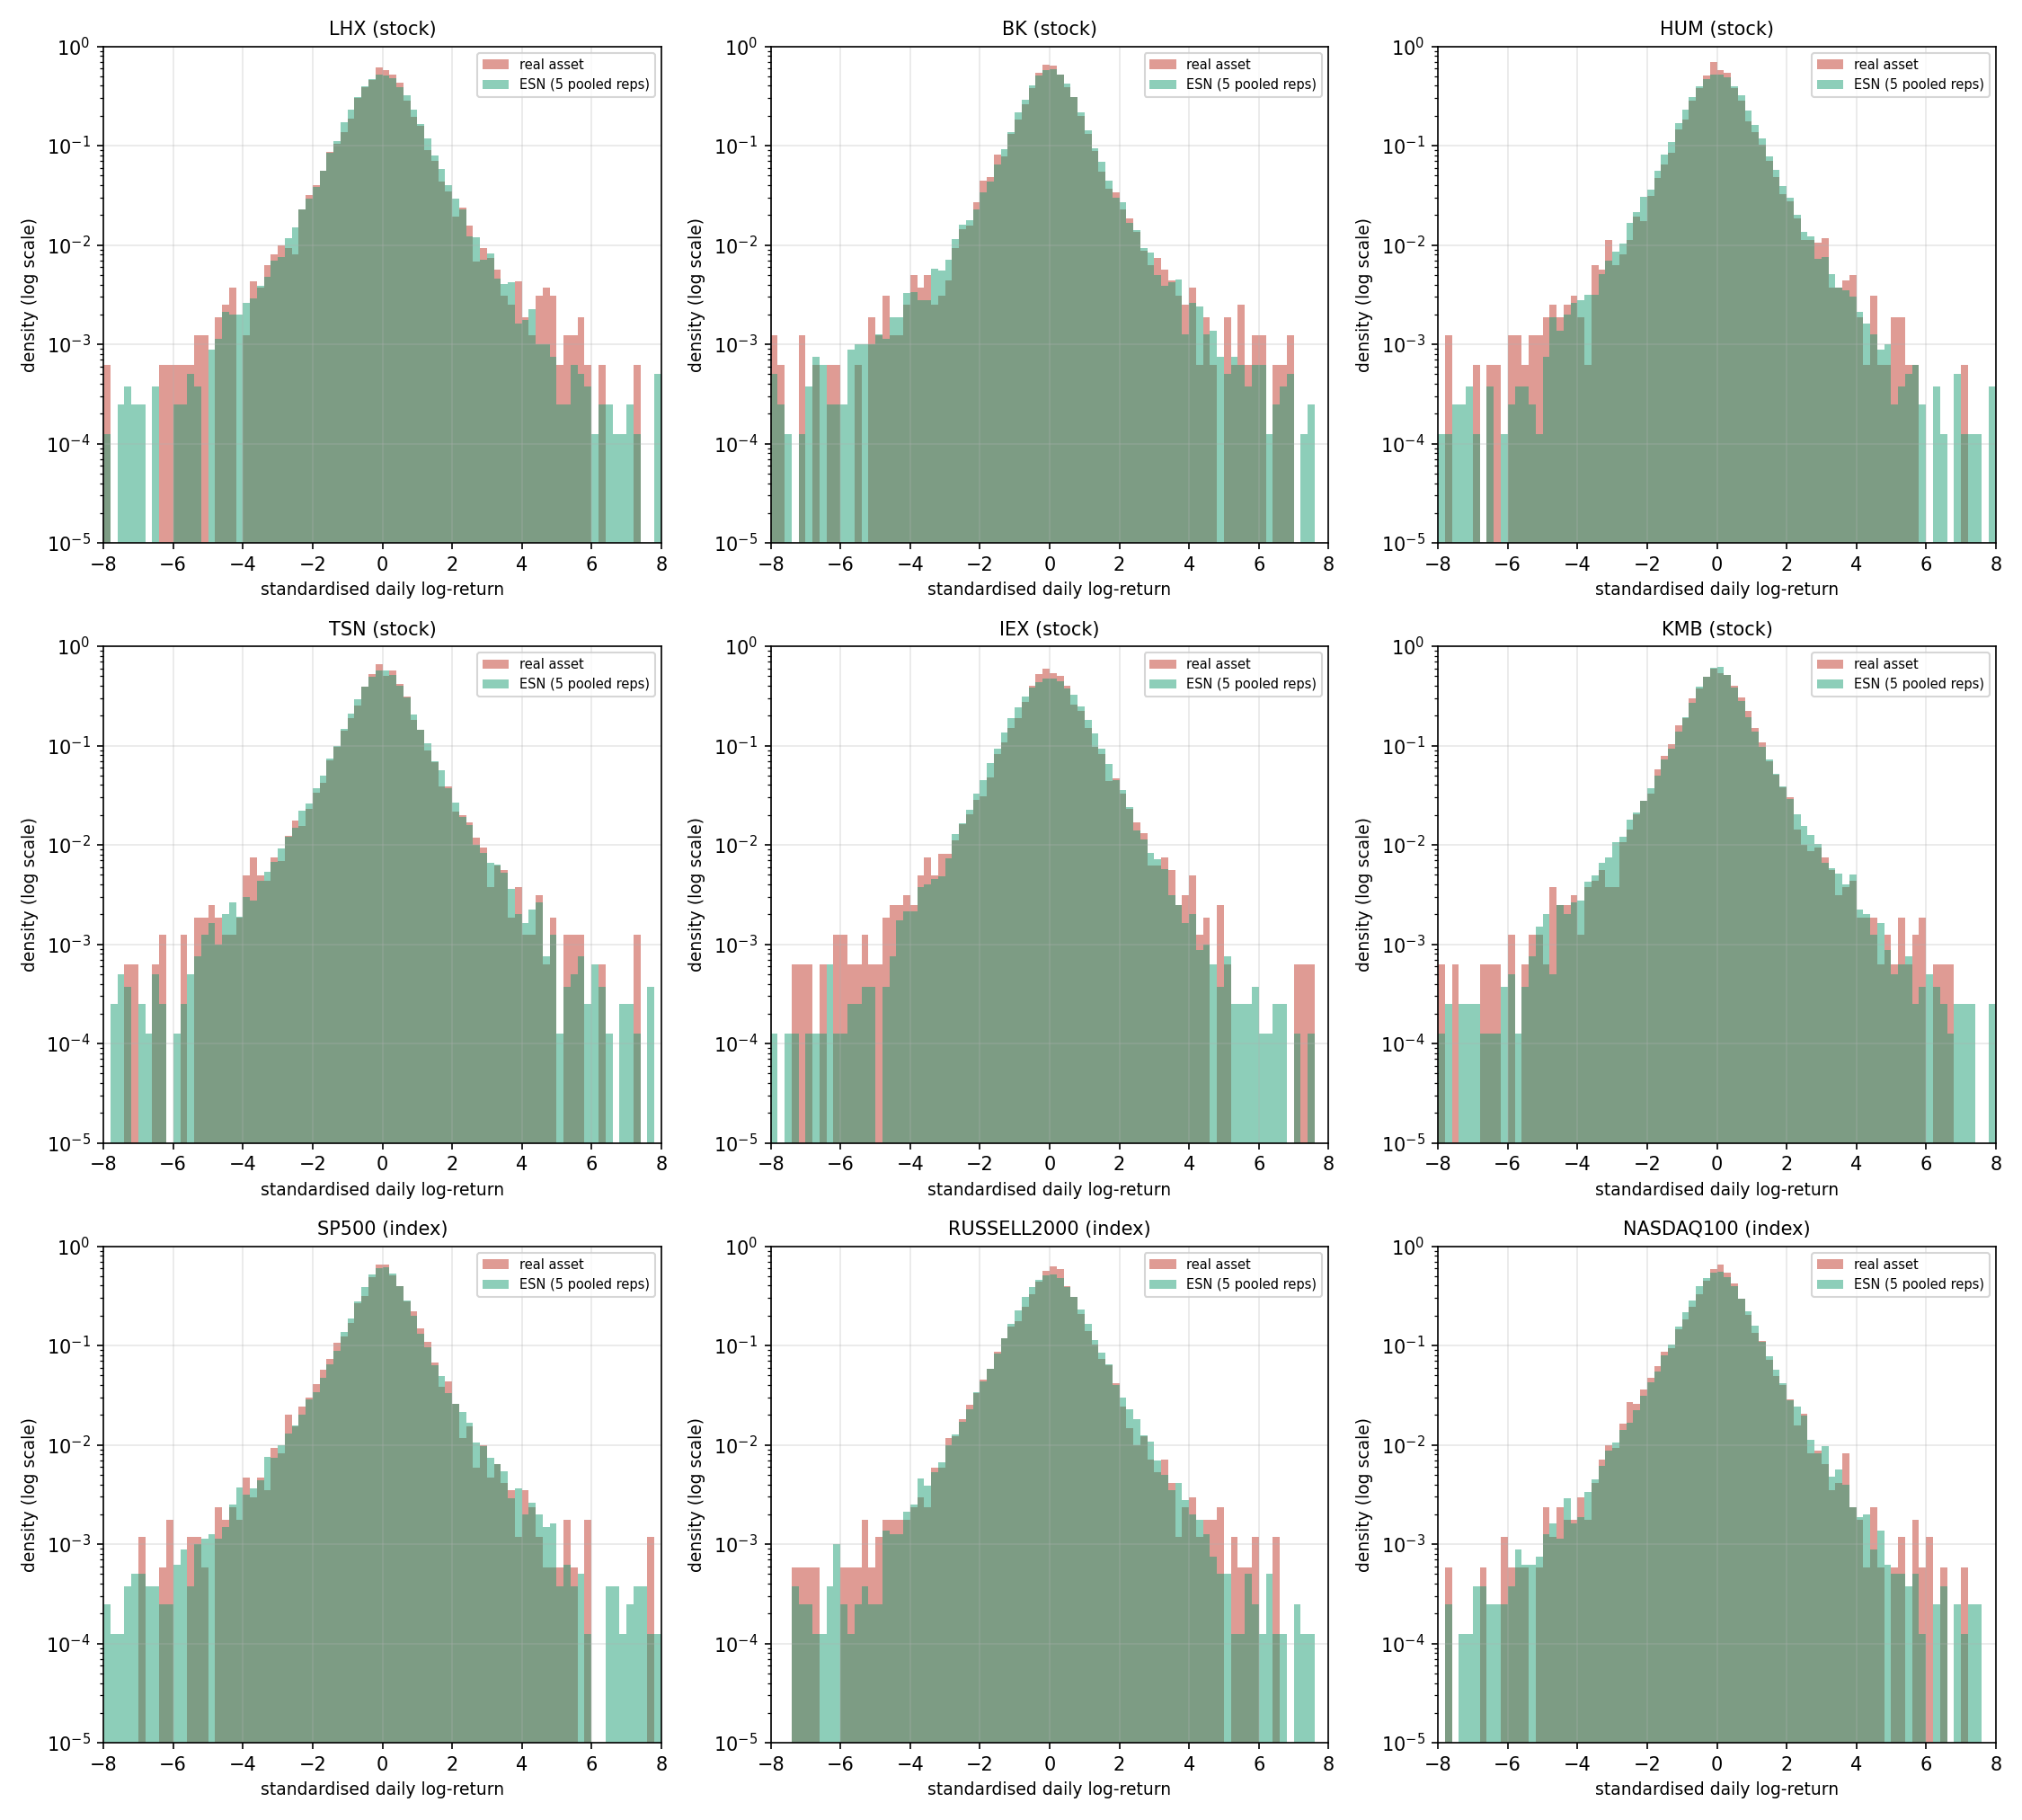
\includegraphics[width=0.98\textwidth]{returns_distribution_bench9.png}
\caption{Empirical distribution of standardised daily log-returns, real
asset vs.\ the calibrated ESN (5 pooled $T=8{,}000$-day replicate paths
per asset, Table~\ref{tab:params}'s own parameters), all 9 assets. Both
series are standardised (mean-subtracted, std-normalised) before
histogramming so shapes, not levels, are compared; the $y$-axis uses a
log scale to make tail behaviour visible. The bulk of the distribution
(roughly $|z|<4$) matches closely for every asset -- a direct visual
confirmation of Table~\ref{tab:coverage}'s own perfect kurtosis coverage
-- while the extreme tail ($|z|>5$--$6$) is noisier and occasionally
sparser in the ESN's own pooled sample for several assets
(\texttt{LHX}, \texttt{TSN}, \texttt{IEX} particularly), consistent with
kurtosis being a 4th-moment average that constrains the bulk of the
distribution's own shape without pinning down the rarest, most extreme
tail events.}
\label{fig:returnsdist}
\end{figure}

\begin{figure}[h]
\centering
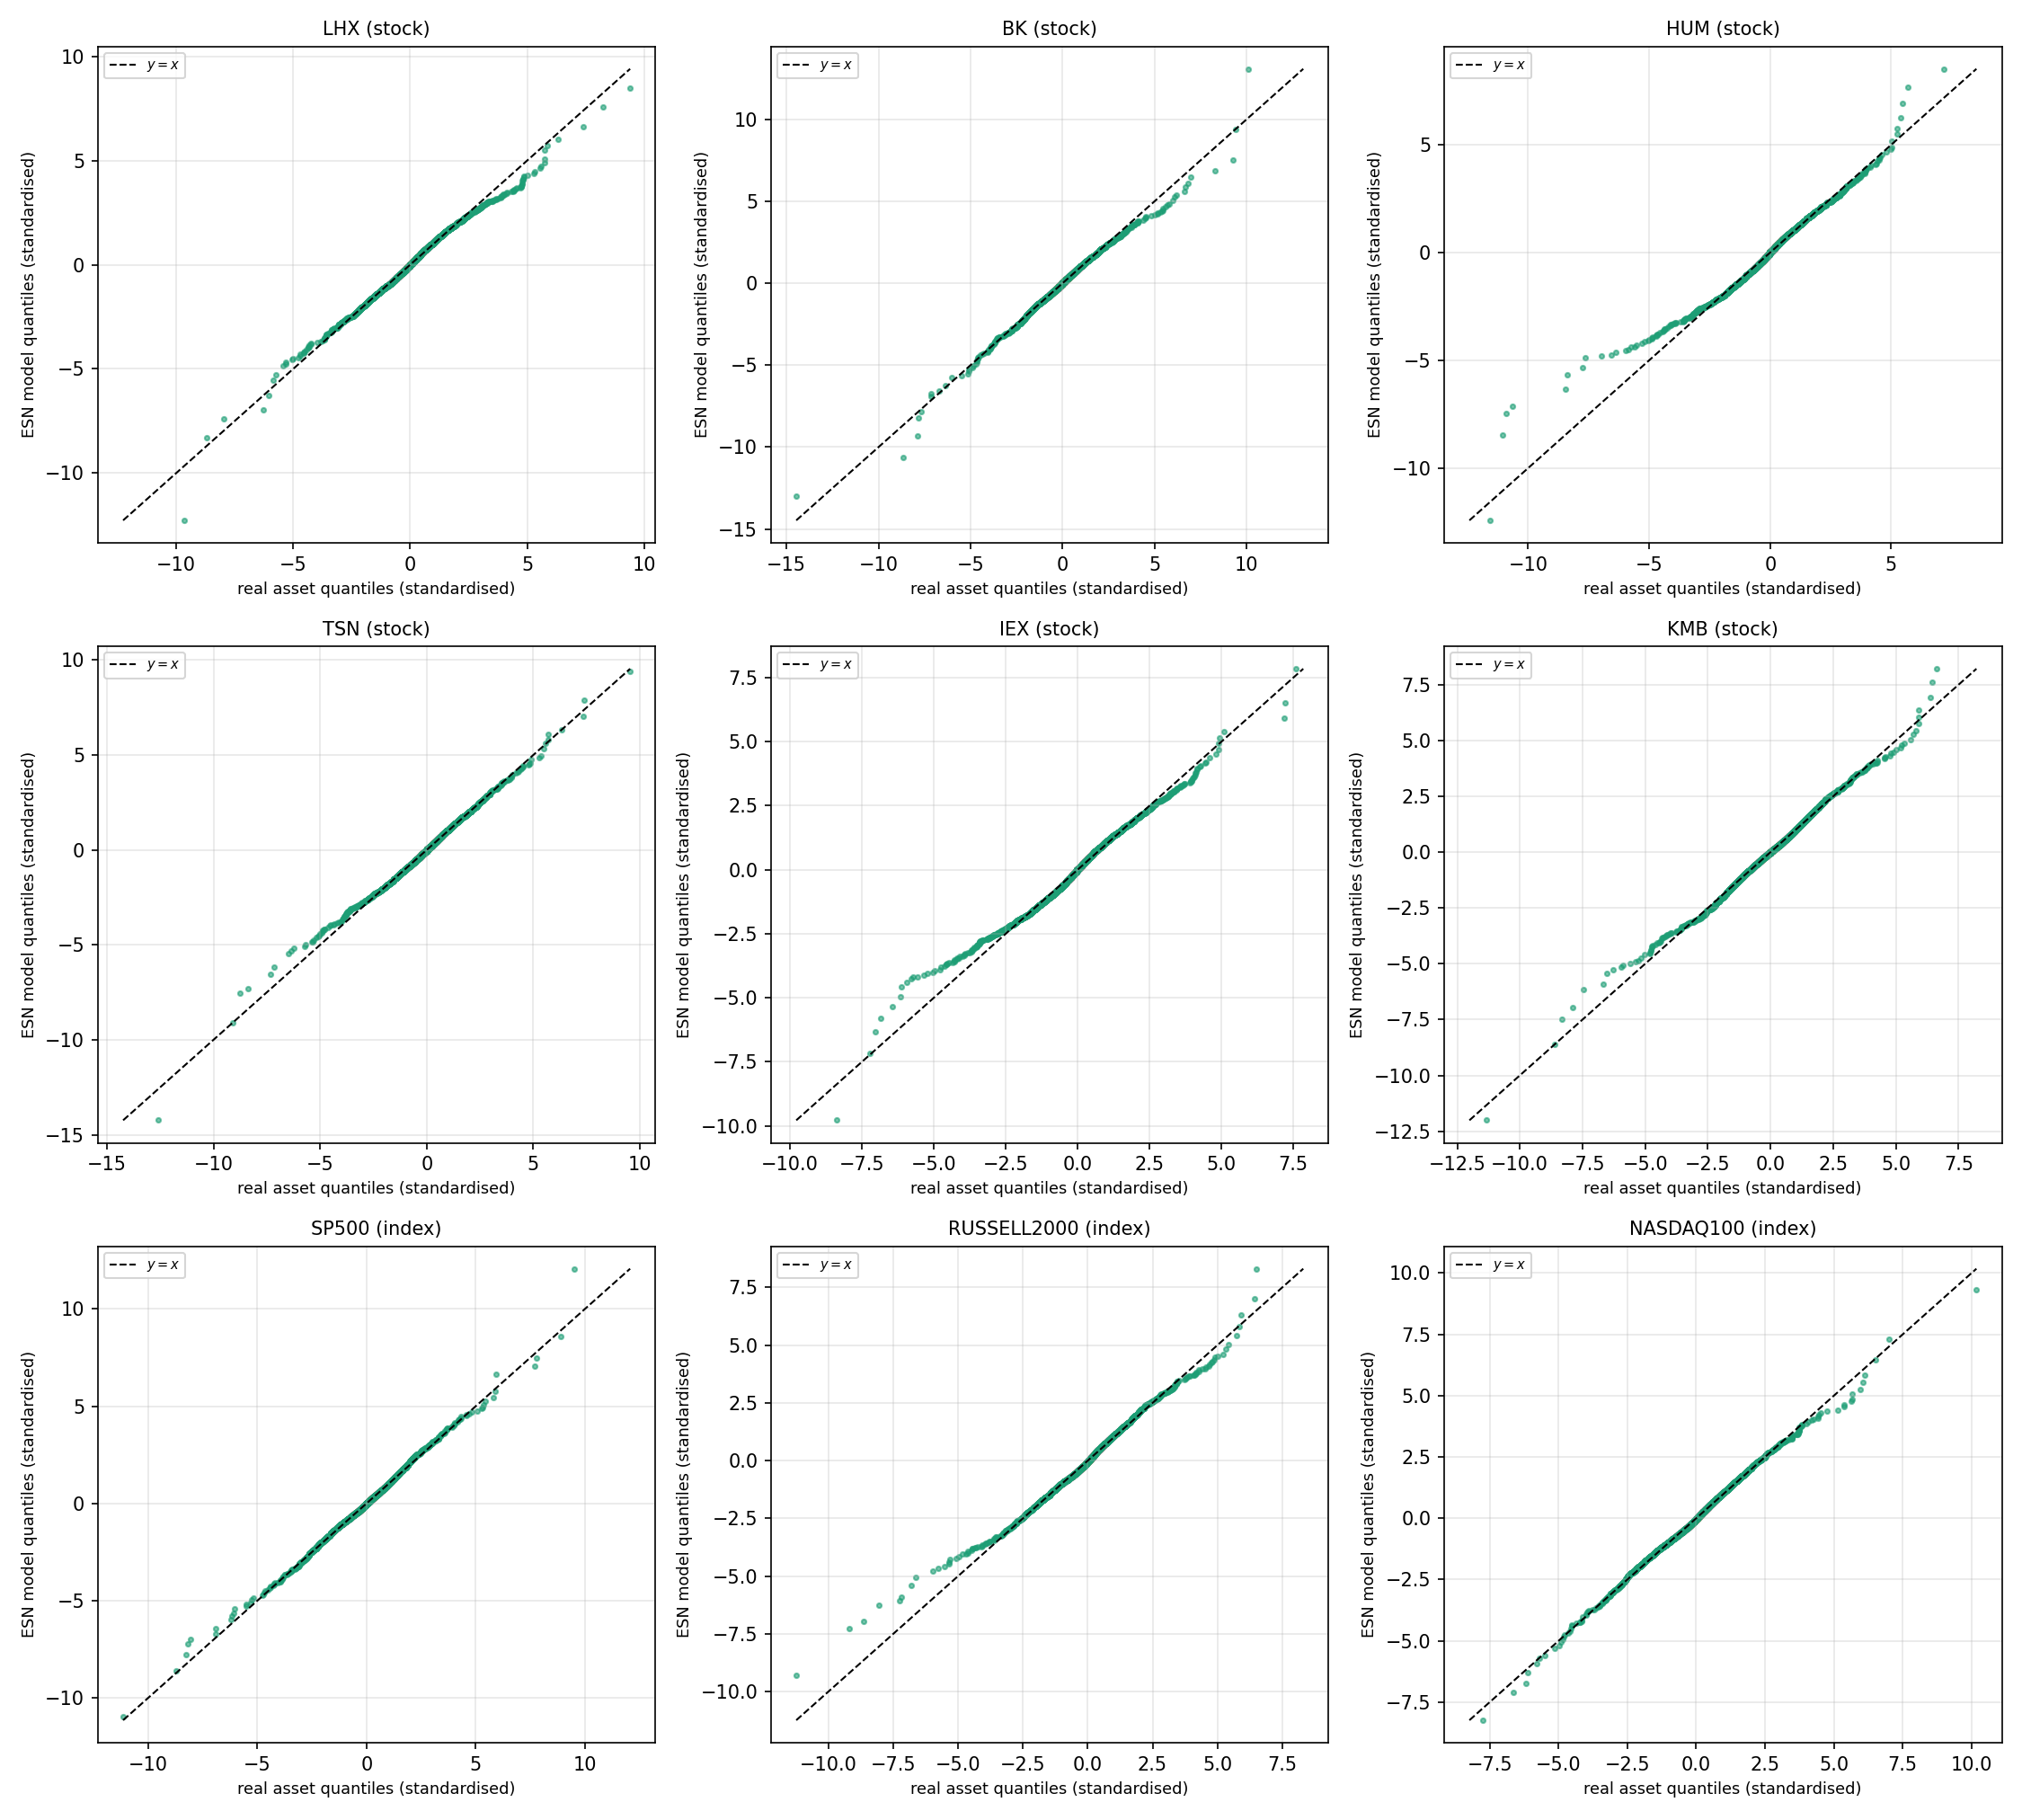
\includegraphics[width=0.98\textwidth]{qq_returns_bench9.png}
\caption{Q--Q plot of standardised daily log-returns, real asset
quantiles (horizontal) vs.\ the calibrated ESN's own quantiles
(vertical, same 5 pooled replicate paths as
Figure~\ref{fig:returnsdist}), all 9 assets; the dashed line is $y=x$.
The bulk of the distribution (roughly $|z|<3$) sits almost exactly on
$y=x$ for every asset, a finer-resolution confirmation of
Figure~\ref{fig:returnsdist}'s own bulk match. The tails reveal a
pattern the histogram does not: for \texttt{LHX}, \texttt{BK},
\texttt{HUM}, \texttt{TSN}, and \texttt{KMB}, the ESN's own negative
tail falls consistently \emph{below} $y=x$ -- the model produces more
extreme downside moves than real data at the same quantile.
\texttt{RUSSELL2000} shows the opposite pattern, with real data's own
negative tail more extreme than the model's. \texttt{SP500} and
\texttt{NASDAQ100} track $y=x$ closely into both tails with only minor
deviation.}
\label{fig:qqplot}
\end{figure}

\FloatBarrier
\begin{table}[h]
\centering
\caption{Coverage: fraction of lags/horizons (or Y/N for the 2 scalar
facts) where the real target falls inside the jointly-calibrated ESN's
own $90\%$ confidence band (40 replicates), all 9 assets.}
\label{tab:coverage}
\begin{tabular}{lccccccc}
\toprule
Asset & type & Hhat & leverage & acf$(|x|)$ & acf$(x^2)$ & Zumbach & kurtosis \\
\midrule
\texttt{LHX}         & stock & Y & $90\%$ & $50\%$ & $67\%$  & $60\%$  & Y \\
\texttt{BK}          & stock & Y & $80\%$ & $67\%$ & $67\%$  & $100\%$ & Y \\
\texttt{HUM}         & stock & Y & $92\%$ & $50\%$ & $50\%$  & $100\%$ & Y \\
\texttt{TSN}         & stock & Y & $38\%$ & $33\%$ & $50\%$  & $60\%$  & Y \\
\texttt{IEX}         & stock & Y & $82\%$ & $33\%$ & $50\%$  & $100\%$ & Y \\
\texttt{KMB}         & stock & Y & $80\%$ & $33\%$ & $83\%$  & $100\%$ & Y \\
\texttt{SP500}       & index & Y & $85\%$ & $67\%$ & $50\%$  & $60\%$  & Y \\
\texttt{RUSSELL2000} & index & Y & $57\%$ & $0\%$  & $0\%$   & $0\%$   & Y \\
\texttt{NASDAQ100}   & index & Y & $78\%$ & $50\%$ & $100\%$ & $100\%$ & Y \\
\bottomrule
\end{tabular}
\end{table}

\textbf{Roughness}: perfect, $9/9$. \textbf{Kurtosis}: perfect, $9/9$.
\textbf{Leverage}: excellent for 8 of 9 assets ($57$--$92\%$), unaffected
by the feedback layer. \textbf{Taylor effect}: recovers substantially --
$33$--$100\%$ for 8 of 9 assets, up from a strict $0$--$17\%$ floor for
every asset in the pure single-signal version. \textbf{Zumbach effect}:
$60$--$100\%$ for 7 of 9 assets, with the qualitative shape now correct
for the same 7 (Figure~\ref{fig:zumbach}). \textbf{\texttt{RUSSELL2000}
is the clear exception}, at $0\%$ on both Taylor curves and Zumbach
despite $57\%$ leverage coverage and perfect roughness/kurtosis.

\section{Limitations and Recommended Next Steps}
\begin{enumerate}
\item \textbf{\texttt{RUSSELL2000} regresses sharply under this
combination}, collapsing to $0\%$ coverage on both Taylor curves and
Zumbach simultaneously. Its own converged $\alpha=0.229$ is not
noticeably more extreme than several assets that succeeded (e.g.\
\texttt{SP500}'s own $0.220$), so the cause is not obviously $\alpha$
itself; whether a different starting point resolves this was not
tested.
\item \textbf{Even where Zumbach's own shape is now correct
(Figure~\ref{fig:zumbach}), the magnitude frequently undershoots}
(\texttt{IEX}, \texttt{RUSSELL2000} particularly, where the ESN's own
mean rises much less steeply than real data). A dedicated per-asset
amplitude correction was not attempted.
\item \textbf{The 3-point smoothing window (\S\ref{sec:smoothing}) and
the feedback layer's own starting value ($\alpha_0=0.1$) were not
themselves tuned}; different choices were not tested against these.
\item \textbf{Common random numbers (\S\ref{sec:crn}) tie the
optimiser's own trajectory to 1 specific noise realisation per asset};
the final confirmation step uses a separate, fixed seed (888) independent
of the optimisation trajectory, but the stage-1 search itself optimises
against 1 realisation, not the true expectation.
\item \textbf{$m_2$ and the $z$-bank's own timescale range and readout
profile remain fixed throughout}; a joint search over a wider parameter
set was not attempted.
\end{enumerate}

\end{document}
